\documentclass{beamer}

\usefonttheme{professionalfonts} % using non standard fonts for beamer
\usefonttheme{serif} % default family is serif

\usepackage{hyperref}
%\usepackage{minted}
\usepackage{animate}
\usepackage{graphicx}
\def\Put(#1,#2)#3{\leavevmode\makebox(0,0){\put(#1,#2){#3}}}
\usepackage{colortbl}
\usepackage{tikz}
\usepackage{amssymb}
\usepackage{enumerate}
\usepackage{arydshln}
\usepackage{algorithm}
\usepackage{algpseudocode}

\colorlet{lightred}{red!25}
\colorlet{lightgreen}{green!25}
\beamertemplatenavigationsymbolsempty

\newcommand\blfootnote[1]{%
  \begingroup
  \renewcommand\thefootnote{}\footnote{#1}%
  \addtocounter{footnote}{-1}%
  \endgroup
}

\makeatletter

%% Textclass specific LaTeX commands.
\newcommand\makebeamertitle{\frame{\maketitle}}%
\AtBeginDocument{%
  \let\origtableofcontents=\tableofcontents
  \def\tableofcontents{\@ifnextchar[{\origtableofcontents}{\gobbletableofcontents}}
  \def\gobbletableofcontents#1{\origtableofcontents}
}
%% User specified LaTeX commands.
\usetheme{Malmoe}
\useoutertheme{infolines}
\addtobeamertemplate{headline}{}{\vskip2pt}
\setbeamercovered{transparent}

\makeatother

%%%%%%%%%%%%%%%%%%%%%%%%%%%%%%%%%%%%%%
%% Main document
%%%%%%%%%%%%%%%%%%%%%%%%%%%%%%%%%%%%%%
\begin{document}
\title[PFLOCK report]{PFLOCK Report}
\author[AC]{Andres Calderon}
\institute[Spring'20]{University of California, Riverside}
\makebeamertitle
\newif\iflattersubsect

\AtBeginSection[] {
    \begin{frame}<beamer>
    \frametitle{Outline} 
    \tableofcontents[currentsection]  
    \end{frame}
    \lattersubsectfalse
}

\AtBeginSubsection[] {
    \begin{frame}<beamer>
    \frametitle{Outline} 
    \tableofcontents[currentsubsection]  
    \end{frame}
}

\begin{frame}{I was wrong...}
    \centering
    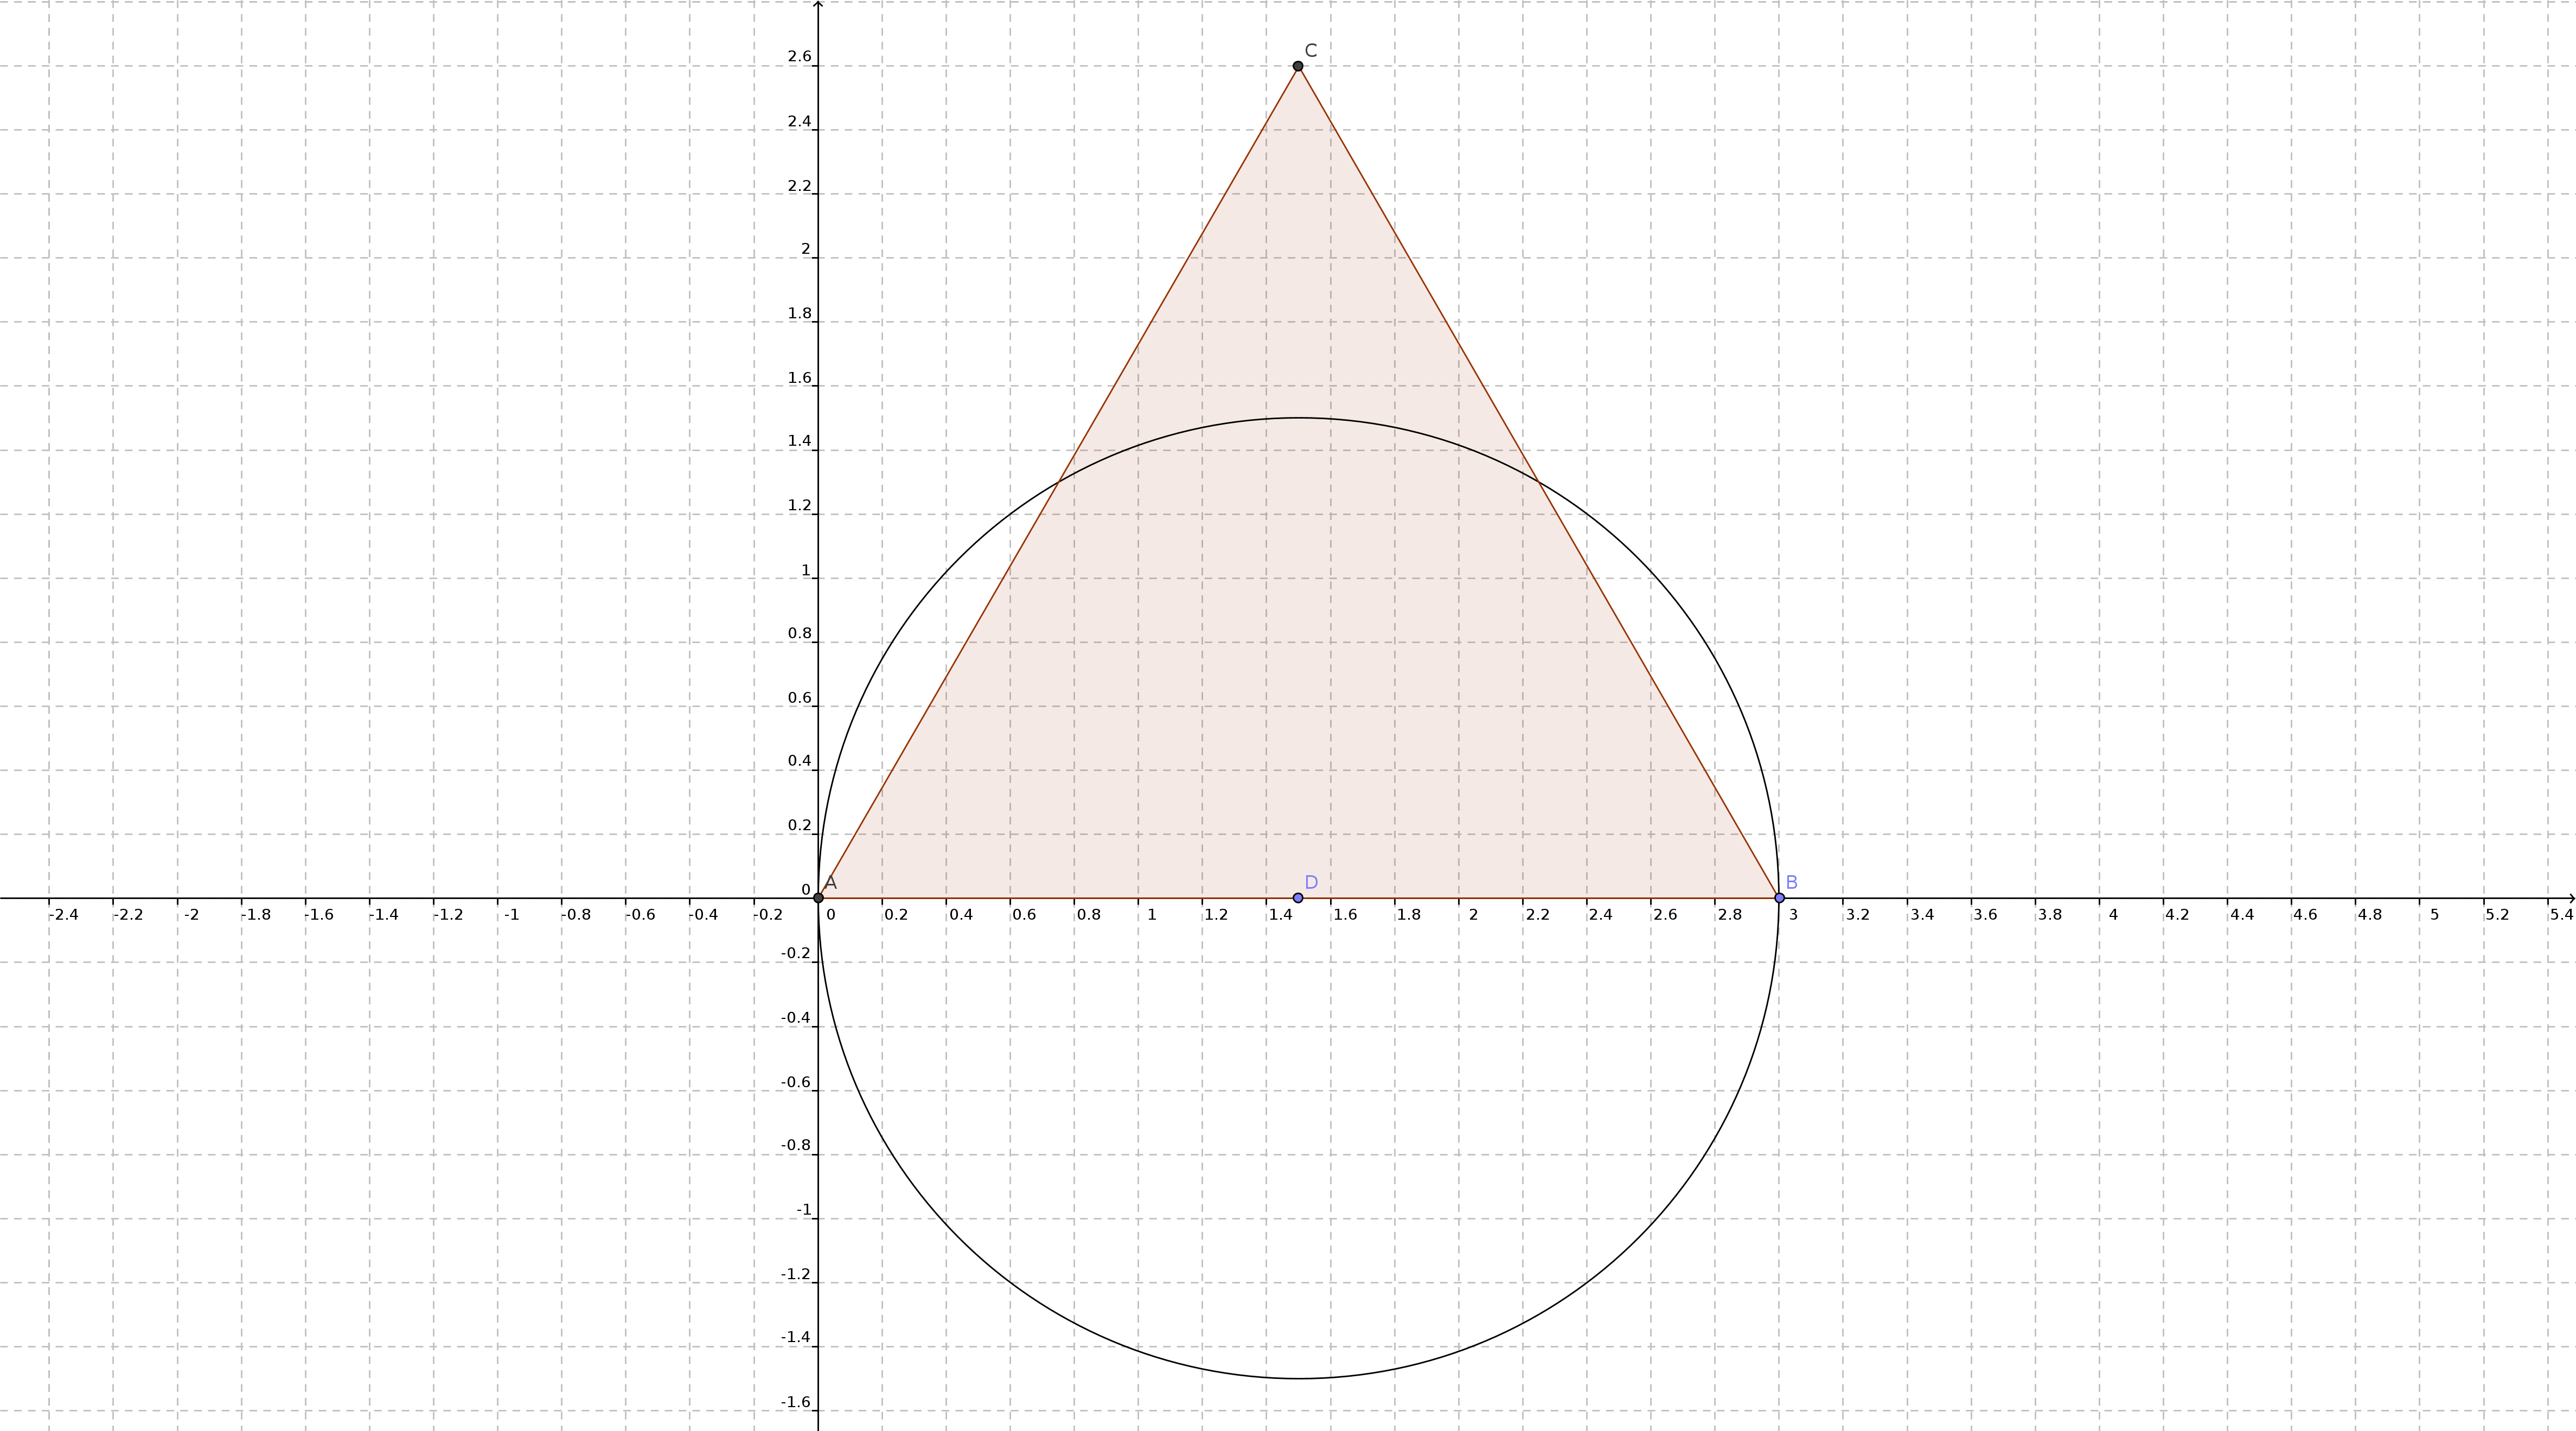
\includegraphics[width=0.6\textwidth]{figures/wrong} \\
    However, finding triangles, or much better cliques, could be very useful...
\end{frame}

\begin{frame}{Maximal cliques instead of just triangles}
    \begin{itemize}
        \item A \textbf{clique}, $C$, in an undirected graph $G = (V, E)$ is a subset of the vertices, $C \subseteq V$, such that every two distinct vertices are adjacent.
        \item A \textbf{maximal clique} is a clique that cannot be extended by including one more adjacent vertex, that is, a clique which does not exist exclusively within the vertex set of a larger clique.
    \end{itemize}
\end{frame}

\begin{frame}{Maximal cliques instead of just triangles}
    \centering
    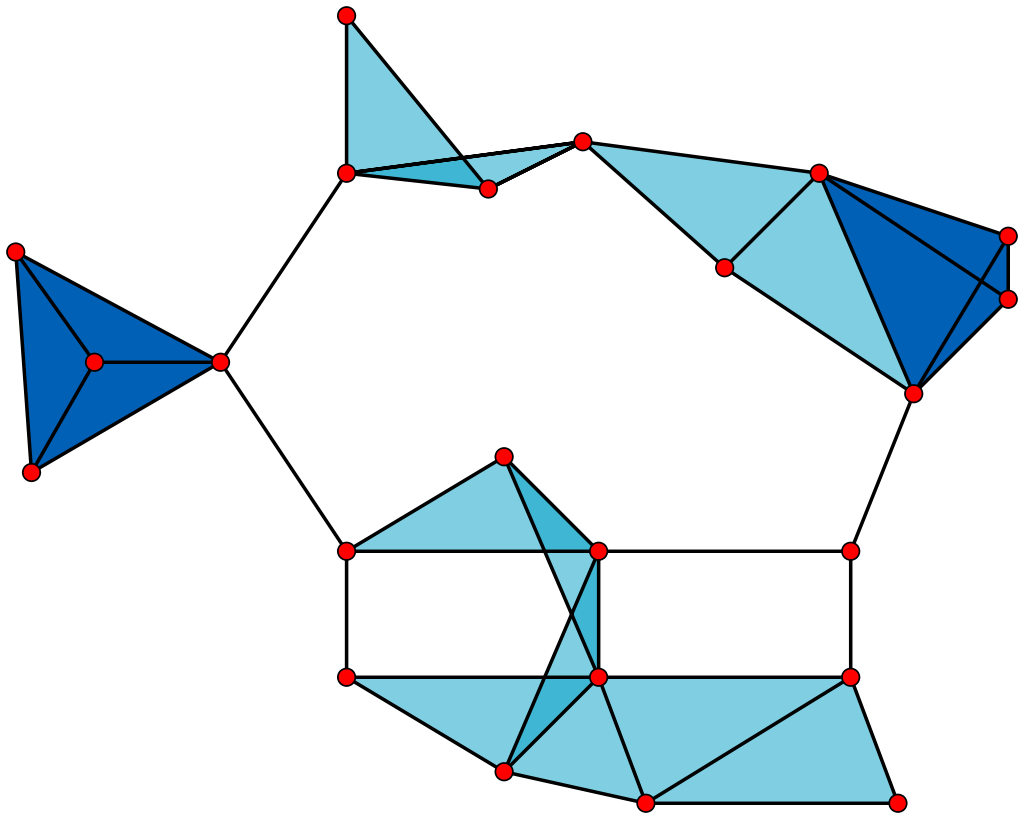
\includegraphics[width=0.75\textwidth]{figures/cliques}
\end{frame}

\begin{frame}{A maximal cliques based approach}{Set of points}
    \centering
    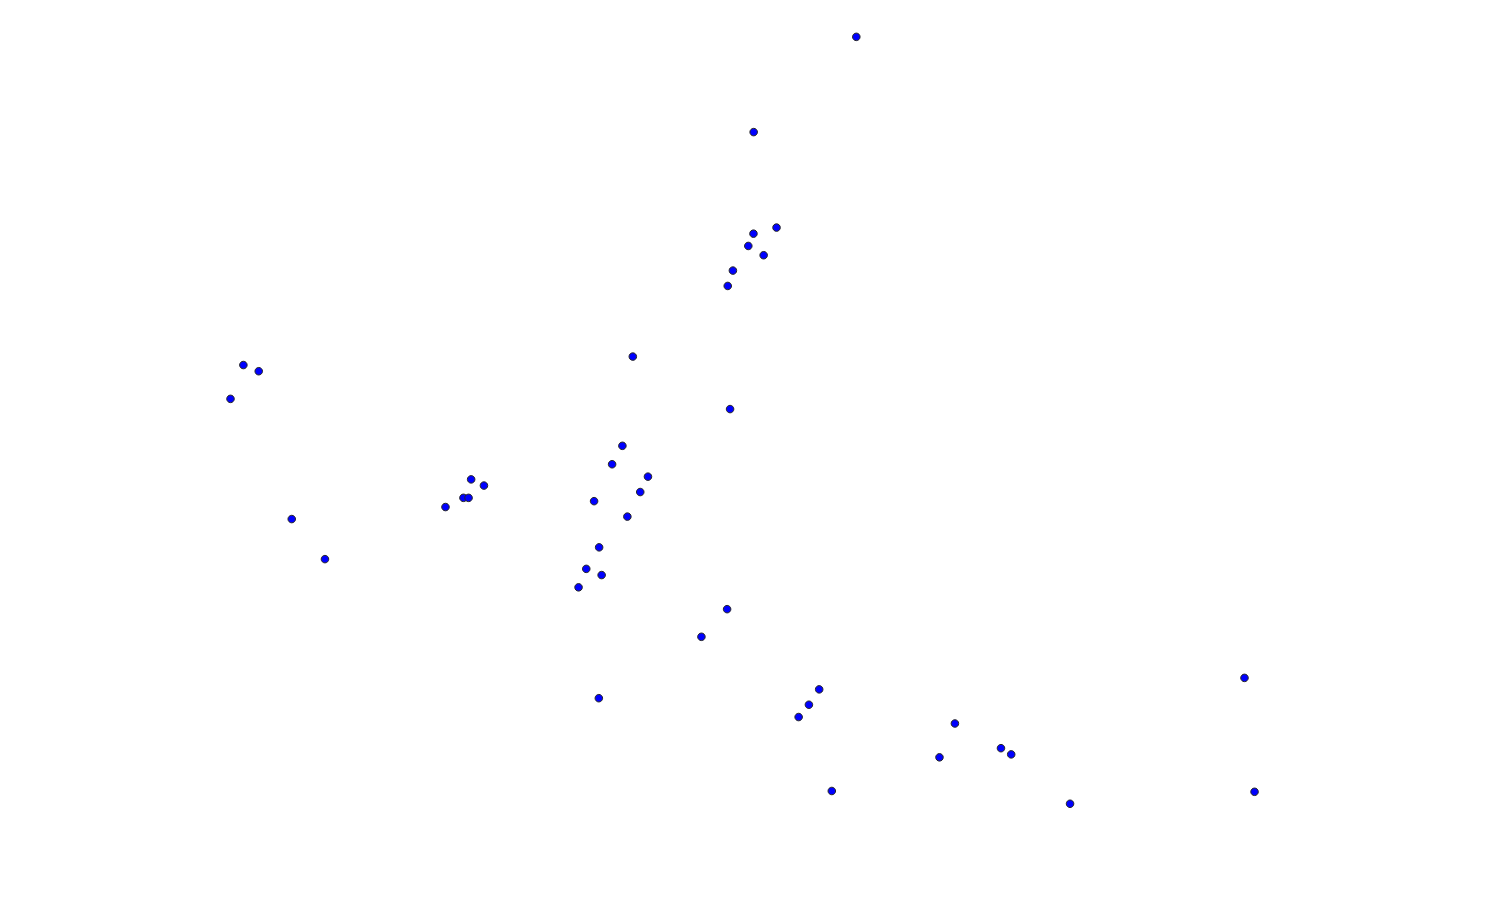
\includegraphics[width=0.85\textwidth]{figures/demo1}
\end{frame}
\begin{frame}{A maximal cliques based approach}{Finding pairs}
    \centering
    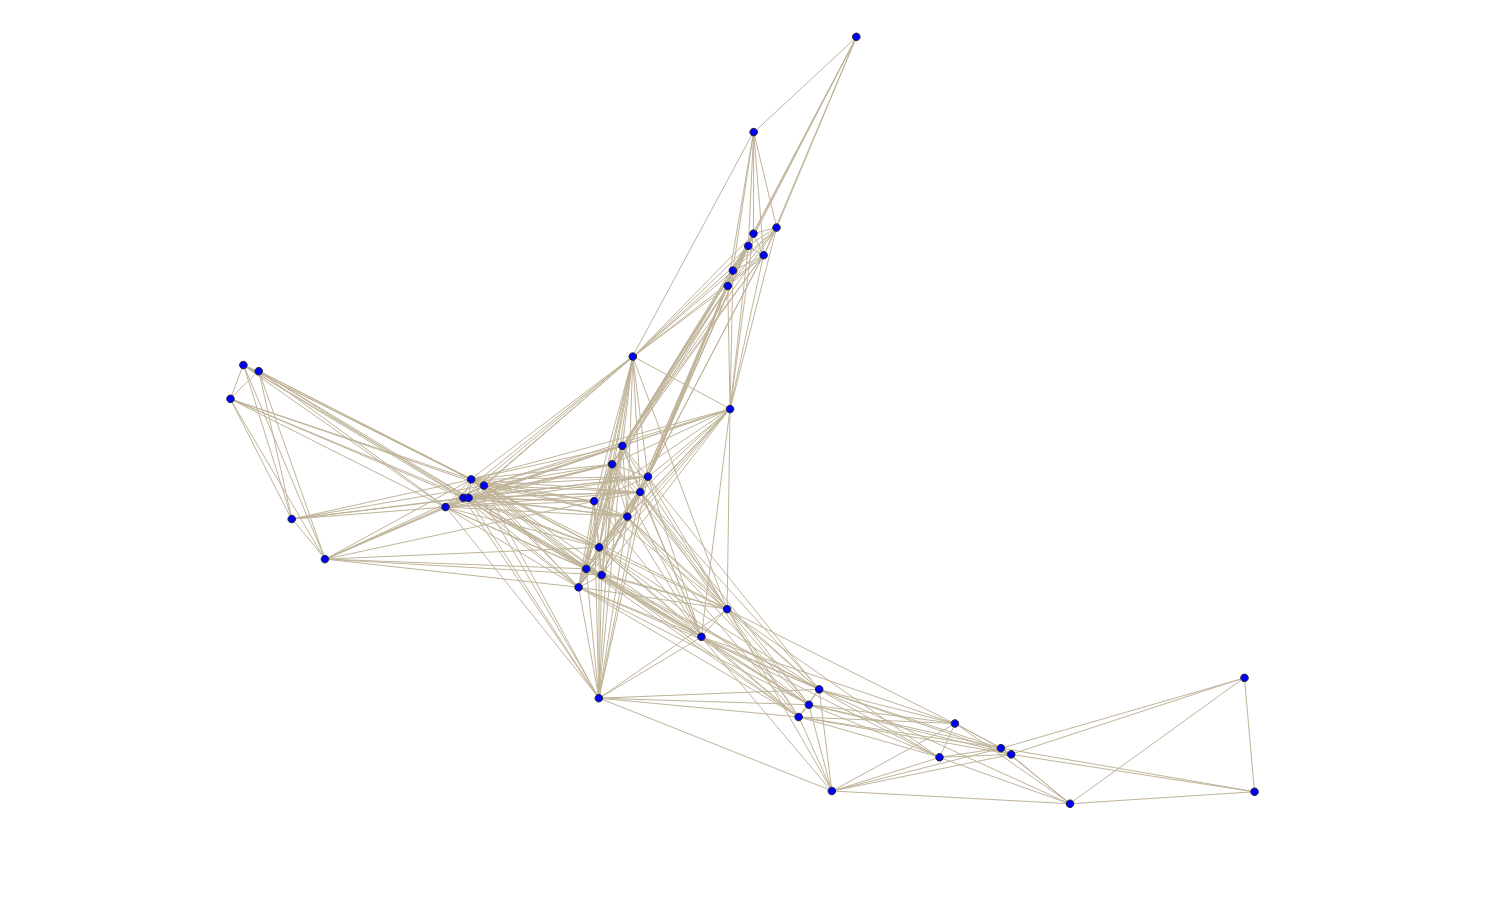
\includegraphics[width=0.85\textwidth]{figures/demo2}
\end{frame}
\begin{frame}{A maximal cliques based approach}{Finding maximal cliques}
    \centering
    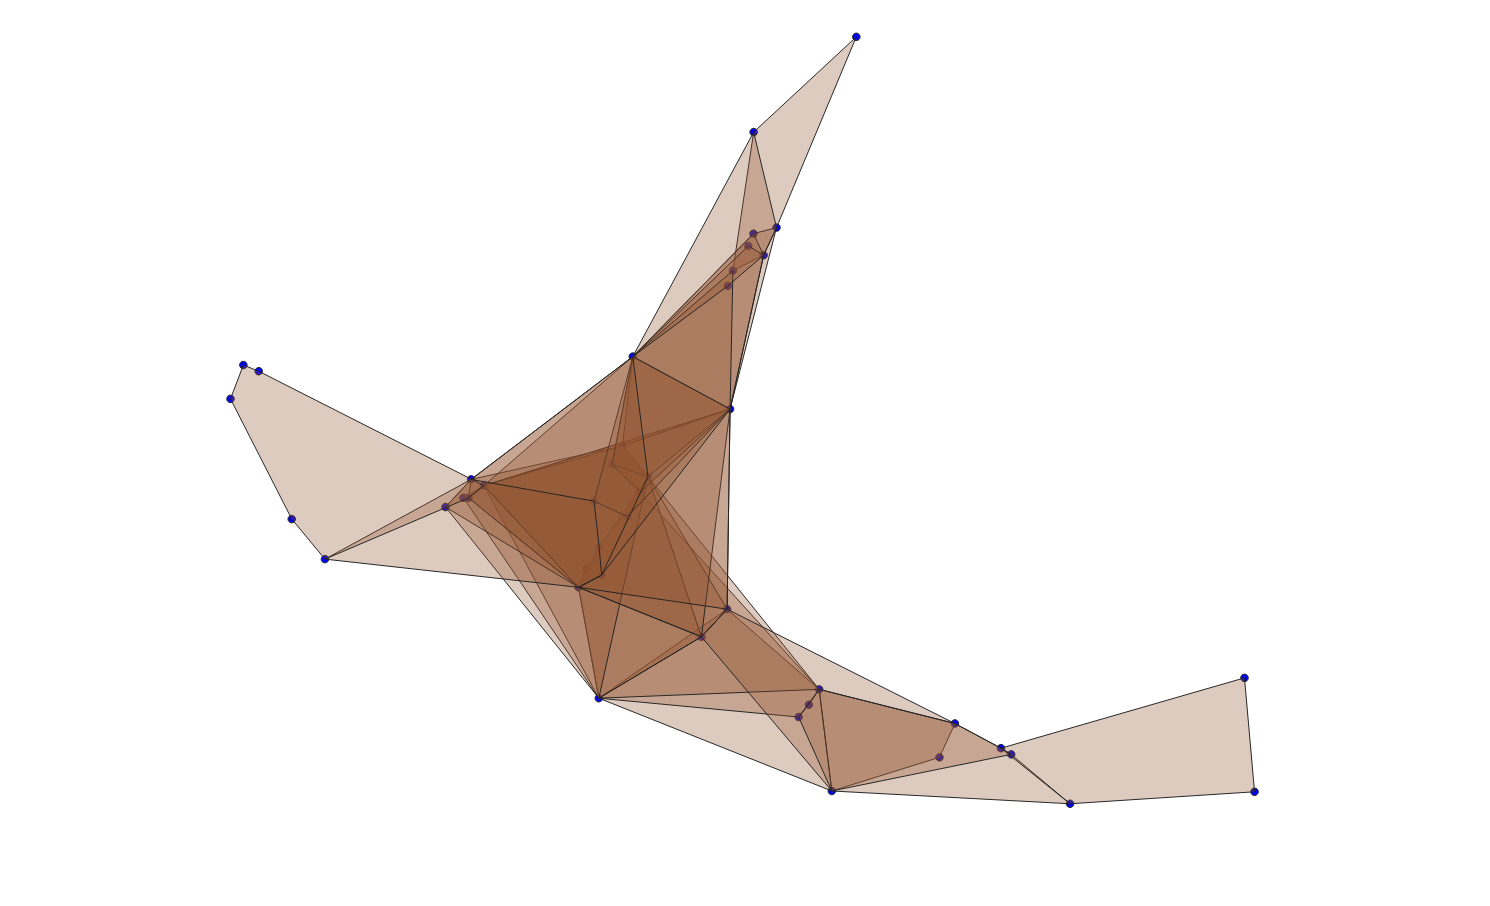
\includegraphics[width=0.85\textwidth]{figures/demo3}
\end{frame}
\begin{frame}{A maximal cliques based approach}{Getting minimum bounding circles}
    \centering
    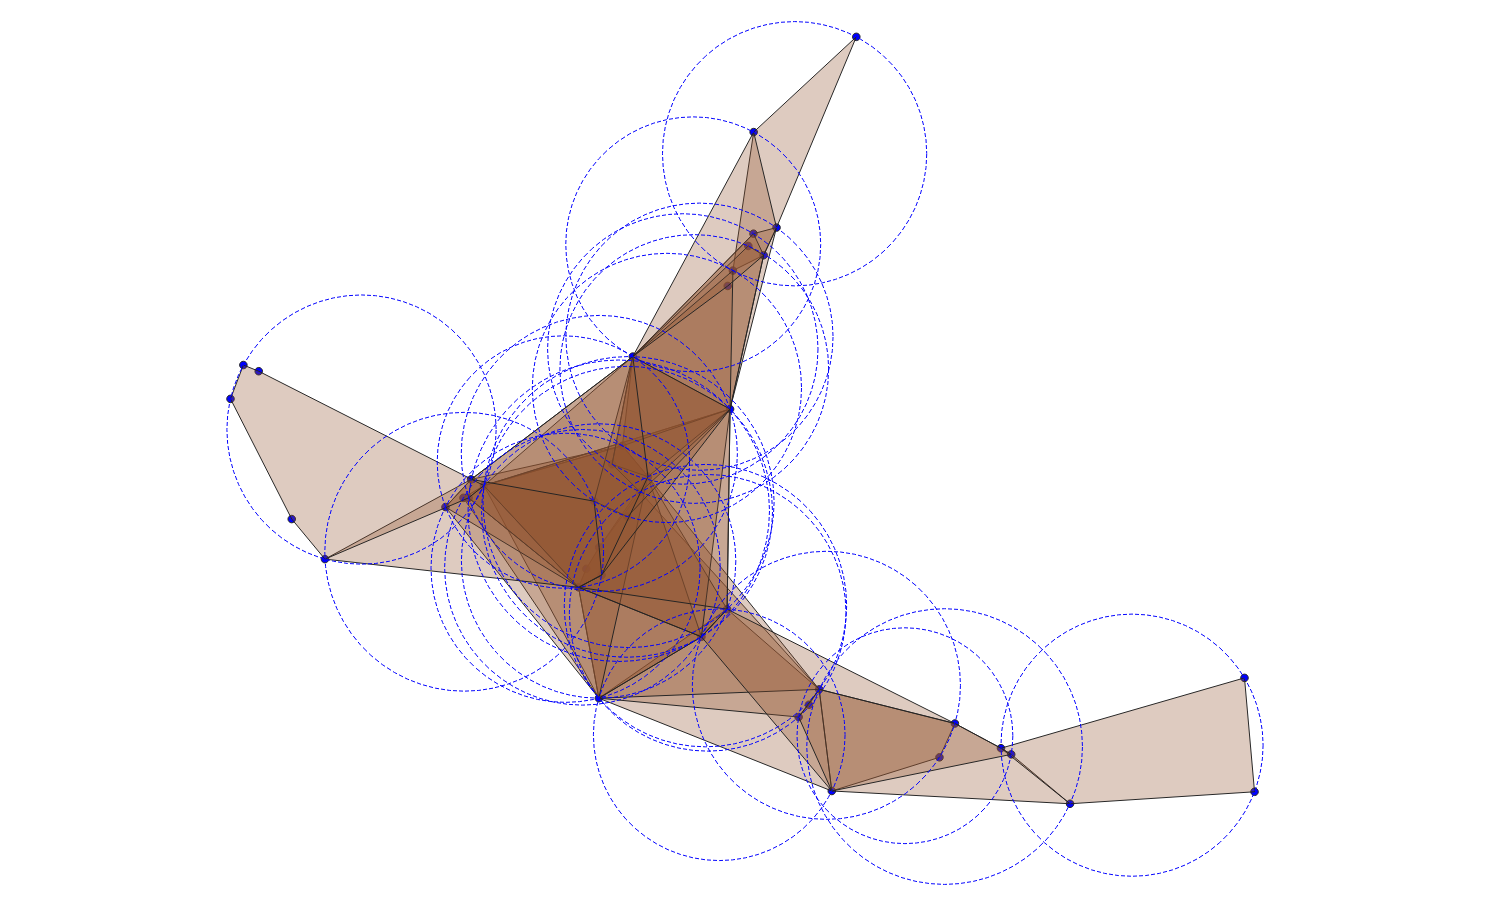
\includegraphics[width=0.85\textwidth]{figures/demo4}
\end{frame}

\begin{frame}{Important notes}
    \begin{itemize}
        \item It is required to perform additional processing if the radius of the minimum bounding circle is greater than $\frac{\varepsilon}{2}$.  
        \item The cost of finding maximal cliques could be high (worst case $O(3^{\frac{n}{3}})$) but many algorithms reports to be practical in real-life graphs.
        \item The reduction on the number of candidate circles is significant (i.e. from 37272 to $\approx$1139 in just 0.804s). 
    \end{itemize}
\end{frame}

\begin{frame}{A maximal cliques based approach}{A large demo}
    \centering
    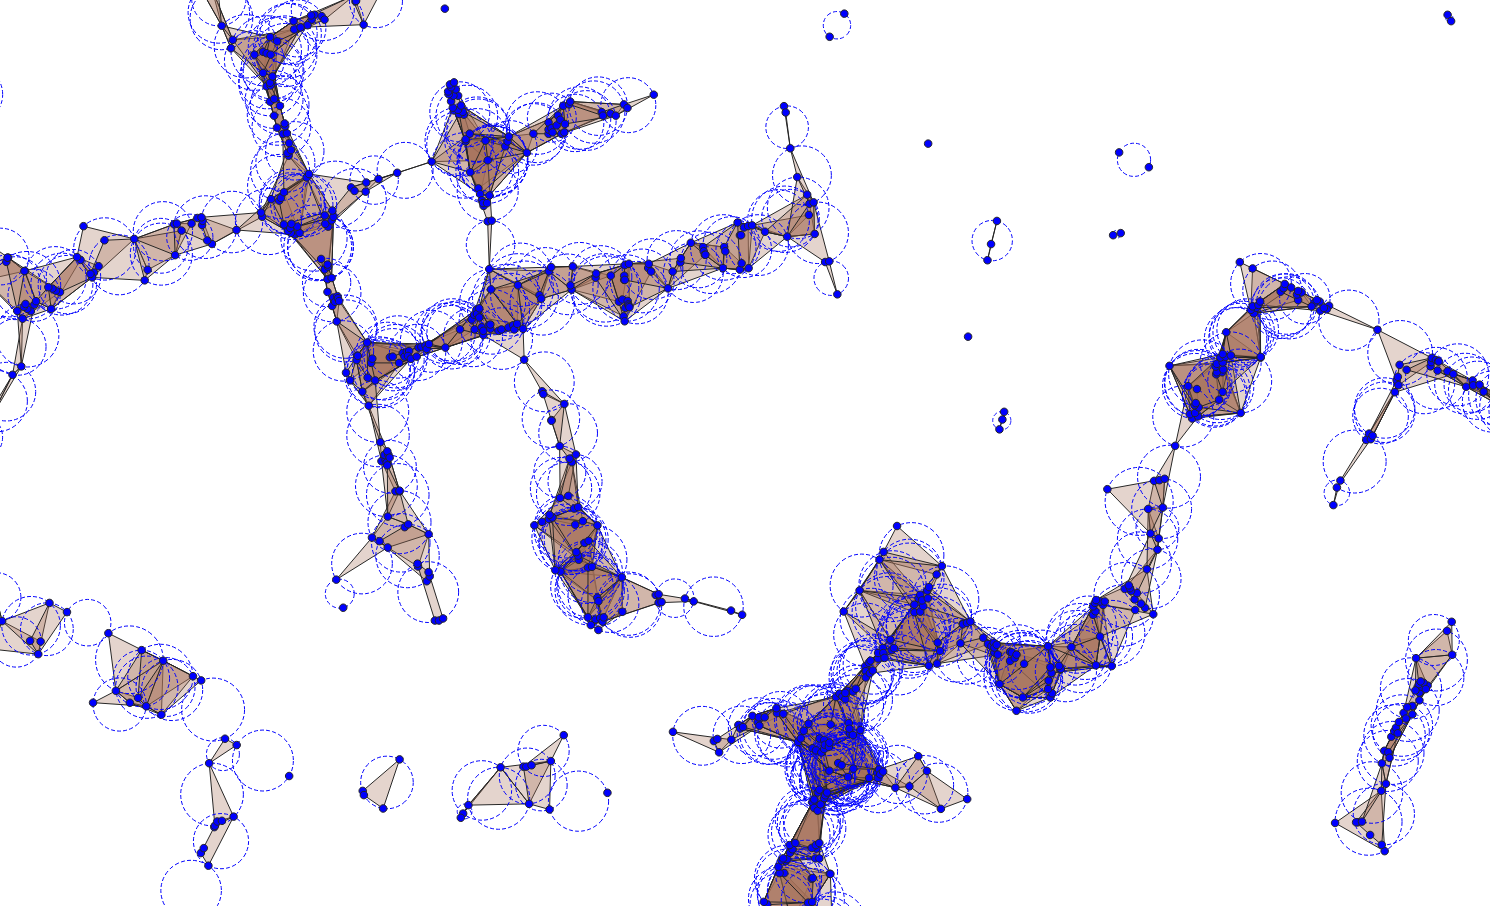
\includegraphics[width=0.85\textwidth]{figures/demo5}
\end{frame}

\end{document}

